\documentclass[]{article}
\usepackage[spanish.mexico]{babel}
\usepackage[T1]{fontenc}
\usepackage[utf8]{inputenc}
\usepackage{lmodern}
\usepackage[a4paper]{geometry}

%\usepackage{natbib}
\usepackage{cite}


%Grafico de barras
\usepackage{pgfplots}

%Graficos e imagenes
\usepackage{graphicx}

\usepackage{wrapfig}

\usepackage{float}%FIJAR IMAGNES con H


%URL
\usepackage{hyperref}


%ONDA EM
\usepackage{tikz,bm}
\usepackage[raggedrightboxes]{ragged2e}

%MATRICES
\usepackage{amsmath}

\title{Apuntes Acústica y Óptica}
\author{Pablo Vivar Colina}
\date{Enero 2021}

%%\usepackage[top=2cm,bottom=2cm,left=1cm,right=1cm]{geometry}


\begin{titlepage}
     \begin{center}
	
\includegraphics[width=0.09\textwidth]{UNAM}\Large Universidad Nacional Autónoma de México
        	
\includegraphics[width=0.09\textwidth]{FI}\\[1cm]
        \Large Facultad de Ingeniería\\[1cm]
       % \Large División de Ciencias Básicas\\[1cm]
         \Large Laboratorio de Fundamentos de Control(6655)\\[1cm]
         %la clave antes era:4314
         \footnotesize Profesor: Salcedo Ubilla María Leonor Ing.\\[1cm]
        \footnotesize Semestre 2019-1\\[1cm]
        
       

        \Large Práctica No. 1\\[1cm]
        
           

\Large Introdcción MATLAB
        
         %Texto a la derecha
          \begin{flushright}
\footnotesize  Grupo 2\\[0.5cm]
\footnotesize Brigada: 4\\[0.5cm]
\footnotesize Rodrigo Adrián Martínez López\\[0.5cm]
\footnotesize Vivar Colina Pablo\\[0.5cm]
 \end{flushright}
    %Texto a la izquierda
          \begin{flushleft}
        \footnotesize Ciudad Universitaria Agosto de 2018.\\
          \end{flushleft}
         
          
        %\vfill
        %\today
   \end{center}
\end{titlepage}
 %agregar portada

\begin{document}

\maketitle

\tableofcontents  % Write out the Table of Contents

\listoffigures  % Write out the List of Figures

\section{Campos Onda Electromagnética}


Sean:\\

\begin{equation}
 \hat{E}(z,t)=E_0\hat{i}e^{i(kz-\omega t)}
\end{equation}

\begin{equation}
  \hat{B}(z,t)=B_0\hat{j}e^{i(kz-\omega t)}
\end{equation}

Nota:\\

\begin{equation}
k=\frac{2 \Pi}{\lambda}
\end{equation}

\begin{equation}
\omega = 2 \Pi f
\end{equation}

\begin{equation}
\frac{\omega}{k}=\lambda f = c
\end{equation}

Expresiones de los campos en polarización lineal:\\



\subsection{Propagación de Ondas Electromagnéticas}

\begin{figure}
	\centering
\begin{tikzpicture}[x={(-10:1cm)},y={(90:1cm)},z={(210:1cm)}]
% Axes
\draw (-1,0,0) node[above] {$z$} -- (5,0,0);
\draw (0,0,0) -- (0,2,0) node[above] {$y$};
\draw (0,0,0) -- (0,0,2) node[left] {$x$};
% Propagation
%\draw[->,ultra thick] (5,0,0) -- node[above] {$c$} (6,0,0);
% Waves
\draw[thick] plot[domain=0:4.5,samples=200] (\x,{cos(deg(pi*\x))},0);
\draw[red,thick] plot[domain=0:4.5,samples=200] (\x,0,{cos(deg(pi*\x))});
% Arrows
%\foreach \x in {0.1,0.3,...,4.4} {
%	\draw[->,help lines] (\x,0,0) -- (\x,{cos(deg(pi*\x))},0);
%	\draw[->,help lines] (\x,0,0) -- (\x,0,{cos(deg(pi*\x))});
%		}
	 Labels
	\node[above right] at (0,1,0) {$\bm{E}$};
	\node[below] at (0,0,1) {$\bm{B}$};
	\end{tikzpicture}
	
\end{figure}


\subsection{Ley de Faraday}

\begin{flushleft}
	
\end{flushleft}

%$\nabla \times \hat{E}=$
%\[
%\begin{matrix}
%	i & j & k\\
%	$\frac{\partial}{\partial x}$ & $\frac{\partial}{\partial y}$ & $\frac{\partial}{\partial z}$\\
%	$E_0e^{i(kz- \omega t)}$ & 0 & 0  
%\end{matrix}
%\]


El resultado de la matriz anterior es

\begin{equation}
\nabla \times \hat{E}=E_0ik\hat{j}e+-\frac{\partial}{\partial t}(B_0\hat{j}e^{i(kz - \omega t)})=B_0 \omega i \hat{j} e^{i(kt-\omega t)}
\end{equation}


\subsection{Anexo}

\begin{equation}
\hat{E}=\frac{\hat{F}}{q}
\end{equation}

\begin{equation}
\hat{F_q}=q\hat{v}=\hat{B}
\end{equation}

\begin{equation}
E_E=\frac{1}{2}=cv^2
\end{equation}

\begin{equation}
   c=\frac{f_0 A}{z}
\end{equation}

Si $|\hat{E}|$ es constante entonces:\\

\begin{equation}
   |\hat{E}|_t=v
\end{equation}

\begin{equation}
   w_b=\frac{1}{2}Li^2
\end{equation}

\begin{equation}
|\hat{B}|=\frac{\mu_0 i N}{t}
\end{equation}


\begin{equation}
L=\frac{\mu_0 N^2 A}{t}
\end{equation}

\subsection{Cálculo de la energía}

\begin{equation}
   W_{EB}=W_E+W_B=\frac{1}{2}(\frac{f_0 A}{z})(Ez)^2+\frac{1}{2}(\frac{\mu_0 N^2 A}{z})(\frac{B z}{\mu_0 N})^2
\end{equation}


\begin{equation}
dW_{EB}=dW_e+dW_b
\end{equation}


\begin{equation}
   dW_{EB}=\frac{1}{2}=f_0AEdt+\frac{1}{2 \mu_0}AB^2dz
\end{equation}


\subsubsection{Potencia Electromagnética}

\begin{equation}
  P_{EB}=\frac{dW_{EB}}{dt}=\frac{1}{2}f_0AEc+\frac{1}{2 \mu_0}AB^2dz
\end{equation}


\subsection{Relación del campo eléctrico y magnético}

\begin{equation}
\frac{E_0}{B_0}=\frac{\omega}{k}=c
\end{equation}

\begin{equation}
   s=\frac{P_{EB}}{A}=\frac{1}{2}f_0E^2c+\frac{1}{2_{m_0}}B^2c
\end{equation}

O también si $\frac{E}{B}=c$

\begin{equation}
   s= \frac{1}{2}f_0EBc^2+\frac{1}{2 \mu_0}EB=\frac{1}{2 \mu_0}[1+f_0 \mu_0c^2]
\end{equation}

\subsection{Módulo de vector de Poynting}

\begin{equation}
   s=\frac{EB}{\mu_0}
\end{equation}

Al final:\\

\begin{equation}
\hat{s}=\frac{\hat{E} \times \hat{B}}{\mu_0}
\end{equation}

\subsubsection{Irradiancia promedio}

\begin{equation}
    |\hat{s}|_{r.m.s.}=\frac{1}{\mu_0}\frac{E_0}{\sqrt{2}} \times \frac{B_0}{\sqrt{2}}=\frac{E_0 B_0}{2 \mu_0} [\frac{W}{m^2}]
\end{equation}

\subsection{Valor RMS}

\begin{equation}
 f(t)=\sqrt{\frac{1}{T} \int_0^T f^2(t)dt}
\end{equation}

$T$ es el periodo total de la función a la cual se le quiere sacar su valor RMS.\\

\section{Ecuación de Onda}



Una ecuación diferencial en derivadas parciales es una ecuación que contiene una o más derivadas parciales de la función indicada. Verifique, por sustitución, que la función:

\begin{equation}
F(x,t)=cos(3x)e^{-2t}
\end{equation}

Satisface la ecuación:

\begin{equation}
F_t=\frac{2}{9}F_{xx}
\end{equation}

Si $F_t$ y $F_{tt}$ denotan las derivadas parciales primera y segunda de $F(x,t)$ con respecto de $t$ y $x$, respectivamente se tiene que:

\begin{equation}
F_t=
\end{equation}


Compruebe directamente, usando la regla de la cadena, que la función:\\

\begin{equation}
f(x,t)=f(x\pm v_pt)
\end{equation}

Donde $v_p$ = constante.\\

Satisface la ecuación de uonda unidimensional $f_{tt}=v^2f_{tt}$

Sea $s(x,t)=x \pm v_p t$, entonces:

\begin{equation}
f_t=\frac{ \partial f}{\partial t},\frac{\partial s}{\partial t}= \pm v_p \frac{\partial f}{\partial s}
\end{equation}

\begin{equation}  
f_u=\frac{\partial}{\partial t} (\pm v_p \frac{\partial f}{\partial s})= \pm v_p \frac{\partial }{\partial s}(\frac{\partial f}{\partial t})=v_p^2 \frac{\partial }{\partial s} (\frac{\partial f}{\partial s})=v_p^2 \frac{\partial^2 f}{\partial s^2}
\end{equation}

Por otro lado:\\

\begin{equation}
f_x=\frac{\partial f}{\partial s},\frac{\partial f}{\partial x}
\end{equation}


\subsection{Ejercicio}

Emplear el métdodo de Fourier para resolver el problema de vibración de una cuerda elástica de longitud L, con extremos fijos sujera a una tensión T, que inicie su movimiento desde el reposo y cuyo perfil en $t=0$ sea $g(x)$

Sua $f(x,t)$ el desplazamiento vertical de un elemento diferencial de cuerda tal que satisfaga la ecuación $f_{tt}=v_p^2 f_{xx}$, con las condiciones iniciales de contorno:\\

\begin{equation}
f(0,t)=f(L,t)=0 (t>0)
\end{equation}


\begin{equation}
f(x,0)=g(x)  (0<x<L)
\end{equation}


\begin{equation}
f_t(x,0)=0   (0<x<T)
\end{equation}

Se propone que la solución $f(x,t)=G(x)H(t)$, que al sustituir en la ecuación resulta:

\subsection{Funciones armónicas}

\subsubsection{Número de onda}

\begin{equation}
k=\frac{2 \Pi}{\lambda}[\frac{1}{m}]
\end{equation}


\subsubsection{Frecuencia angular}

\begin{equation}
\omega = 2 \Pi f=\frac{2 \Pi}{T}[\frac{1}{s}]
\end{equation}

Nota:\\

\begin{equation}
\frac{\omega}{k}=\lambda * f=v
\end{equation}

donde $v$ es la velocidad de propagación de la onda\\

\subsubsection{Onda senoidal}

\begin{equation}
f(x,t)=Asin(x \pm t)
\label{senA}
\end{equation}



\begin{itemize}
	\item $A$ amplitud
\end{itemize}


\begin{equation}
f(x,t)=Asin(k x \pm \omega t)
\label{senB}
\end{equation}


\begin{equation}
f(x,t)=A sin \frac{2 \Pi}{\lambda}( x \pm \lambda f t)
\label{senC}
\end{equation}


\begin{equation}
f(x,t)=A sin \frac{2 \Pi}{\lambda}( x \pm  t)
\label{senD}
\end{equation}

Nota, la expresión \ref{senA} es equivalente con las expresiones \ref{senB}, \ref{senC} y \ref{senD}

La expresión \ref{senB} es solución a $f_{tt}=v^2f_{tt}$ por lo tanto podemos escribir:\\

\begin{equation}
f_t=A \omega sin(kx+ \omega t)
\end{equation}

\begin{equation}
f_{tt}=-A \omega^2 sin(kx+\omega t)
\end{equation}


\begin{equation}
f_x=A k sin(kx+ \omega t)
\end{equation}


\begin{equation}
f_{xx}=-A k^2 sin(kx+\omega t)
\end{equation}

Al final:\\

\begin{equation}
\frac{f_{tt}}{f_{xx}}=\frac{\omega^2}{k^2} =v^2
\end{equation}

La rapidez de una onda en una cuerda se puede obtener mediante la siguiente expresión:\\

\begin{equation}
v=\sqrt{\frac{T}{\mu}}
\end{equation}

La expresión que nos proporciona los modos de vibración es:\\

\begin{equation}
\lambda_n=\frac{2 L}{n}
\end{equation}

Donde $L$ es la longitud de la cuerda, $\lambda es la longitud de onda$ y n son números naturales correspondientes a los modos de vibración.\\

Asimismo se puede obtener la n-ésima frecuencia a ptravés de la fórmula:\\

\begin{equation}
f_n=n(\frac{v_p}{2L})
\end{equation}

\subsection{Ejercicio}

Verifique esprimentalmente que la función armónica:\\

\begin{equation}
g(x,t)=Ae^{i(kx+\omega t)}+Ae^{i(kx-\omega t+\Pi)}
\end{equation}

Con $k=\frac{2 \Pi}{\lambda}$ y $\omega=2 \Pi f$, satisface la ecuación de onda unidimensional.

\subsubsection{Resolución}

Ya que $e^{i\Pi}=-1$,$g(x,t)$ se escribe de la forma:\\

\begin{equation}
g(x,t)=Ae^{ikt}(e^{i \omega t}-e^{-i \omega t})
\end{equation}

Así que, si:\\

\subsection{Apéndice}


\begin{equation}
sin x=\frac{e^{ix}-e^{-ix}}{2i}
\end{equation}

\section{Ondas Electromagnéticas}


\subsection{Interfaz plana, incidencia oblicua}


\begin{figure}[h!]
	\centering
	\begin{tikzpicture}[]
	% Axes
	%\draw
	\draw (-2.5,0) -- (2.5,0);
	\draw (0,-2.5) -- (0,2.5);
	%azules
	\draw (0,0) [blue,thick]  -- (1.5,1);
	\draw (0,0) [blue,thick]  -- (-1,1.5);
	\draw (0,0) [blue,thick]  -- (-1,-1.5);
	%rojos
	\draw (0.86,0.5) [red,thick]  -- (0.6,1);
	\draw (-0.5,0.86) [red,thick]  -- (0.2,1.5);
	\draw (-0.5,-0.86) [red,thick]  -- (-1,-0.4);
	
	Labels
	\node[above] at (0,2.5) {$y$};
	\node[above] at (2.5,0) {$x$};
	\node[below right] at (0,-2.5) {$n_2$};
	\node[below left] at (0,-2.5) {$n_1$};
	
	\node[green, above] at (1,0) {$\gamma$};
	\node[green, above] at (-0.5,0) {$\beta$};
	\node[green, below] at (-0.5,0) {$\alpha$};
	
	\node[red, above] at (0.6,1) {$\bar{E_{03}}$};
	\node[red, above] at (0.2,1.5) {$\bar{E_{02}}$};
	\node[red, above] at (-1,-0.4) {$\bar{E_{01}}$};
	
	\node[blue, above] at (1.5,1) {$\bar{k_3}$};
	\node[blue, above] at (-1,1.5) {$\bar{k_2}$};
	\node[blue, above] at (-1,-1.5) {$\bar{k_1}$};
	\end{tikzpicture}
	\caption{Onda 2D}
\end{figure}

\begin{eqnarray}
\bar{k_1}=k_1[cos \alpha \hat{i} + sin \alpha \hat{j}]\\
\bar{k_2}=k_2[-cos \beta \hat{i} + sin \beta \hat{j}]\\
\bar{k_3}=k_3[cos \gamma \hat{i} + sin \gamma \hat{j}]
\end{eqnarray}

\begin{eqnarray}
\bar{E_{01}}=E_{01}[-sin \alpha \hat{i} + cos \alpha \hat{j}]\\
\bar{E_{02}}=E_{02}[sin \beta \hat{i} + cos \beta \hat{j}]\\
\bar{E_{03}}=E_{03}[-sin \gamma \hat{j} + cos \gamma \hat{j}]
\end{eqnarray}

$r=x\hat{j}+y\hat{j}$ Entonces:\\

\begin{eqnarray}
\bar{E_1}=\bar{E_{01}}e^{i(\bar{k_1}\bar{r}-\omega t)}=E_{01}[-sin \alpha \hat{i} + cos \alpha \hat{j}] e^{i[k_1(x cos \alpha + y sin \alpha)-\omega t]}\\
\bar{E_2}=\bar{E_{02}}e^{i(\bar{k_2}\bar{r}-\omega t)}=E_{02}[sin \beta \hat{i} + cos \beta \hat{j}] e^{i[k_2(x cos \beta + y sin \beta)-\omega t]}\\
\bar{E_3}=\bar{E_{03}}e^{i(\bar{k_3}\bar{r}-\omega t)}=E_{03}[-sin \gamma \hat{i} + cos \gamma \hat{j}] e^{i[k_3(x cos \gamma + y sin \gamma)-\omega t]}
\end{eqnarray}

Así: $\bar{E_1}=\bar{E_2}+\bar{E_3}$ Condición de frontera $E_{1y}+E_{2y}=E_{3y}$\\

Componente tangencial de $\bar{E}$ Entonces:\\

\begin{eqnarray}
E_{01}cos \alpha e^{ik_1y sin \alpha-i \omega t}*e^{-i \omega t}\\
E_{02}cos \alpha e^{ik_2y sin \beta-i \omega t}*e^{-i \omega t}\\
E_{03}cos \alpha e^{ik_3y sin \gamma-i \omega t}*e^{-i \omega t}
\end{eqnarray}


Nota importante para la simplificación $e^a+e^b=e^c$ implica que $a=b$ y $b=c$\\

\begin{eqnarray}
E_{01}cos \alpha e^{ik_1y sin \alpha-i \omega t}\\
E_{02}cos \alpha e^{ik_2y sin \beta-i \omega t}\\
E_{03}cos \alpha e^{ik_3y sin \gamma-i \omega t}
\end{eqnarray}

Al final: $k_1ysin \alpha=k_2y sin \beta$ implicando que $k_1$ y $k_2$ están en el mismo medio por lo tanto son iguales obteniendo que: $sin \alpha=sin \beta$ y por tanto $\alpha=\beta$ y éste resultado es la $Ley$ $de$ $la$ $reflexión$. Además $k_1ysin\alpha=k_3sin \gamma$ sustituyendo podemos llegar a $La$ $Ley$ $de$ $snell$: $n_1 sin \alpha=n_2 sin \gamma$\\

\section{Ecuaciones de Maxwell}



\subsection{Ecuaciones de Maxwell con fuentes}

\begin{equation}
\nabla \hat{E}=\frac{\rho}{f_0}
\label{gauss1}
\end{equation}

\begin{equation}
\nabla \hat{B}=0
\label{gauss2}
\end{equation}

\begin{equation}
\nabla x \hat{E}=-\frac{\partial \hat{B}}{\partial t}
\label{Faraday}
\end{equation}

\begin{equation}
\nabla x \hat{B}=\mu_0 (\hat{J}+\frac{\partial \hat{D}}{\partial t})
\label{Ampere-Maxwell}
\end{equation}

Las ecuaciones \ref{gauss1} y \ref{gauss2} son llamadas ecuaciones de gauss

La ecuación \ref{Faraday} tiene el nombre de ecuación de Faraday.\\


La ecuación \ref{Ampere-Maxwell} tiene el nombre de ecuación de Ampere Maxwell.\\


\subsection{Ecuaciones de Maxwell sin fuentes}

\begin{equation}
\nabla \hat{E}=0
\end{equation}

\begin{equation}
\nabla \hat{B}=0
\end{equation}

\begin{equation}
\nabla x \hat{E}=-\frac{\partial \hat{B}}{\partial t}
\end{equation}

\begin{equation}
\nabla x \hat{B}=\mu_0\hat{J}+\epsilon_0\mu_0\frac{\partial \hat{E}}{\partial{t}}
\end{equation}

\subsection{Ecuación de Onda}

\begin{equation}
\nabla x \nabla x \hat{A}=\nabla(\nabla \hat{A})-\nabla^2\hat{A}
\end{equation}

\begin{equation}
\nabla x (\frac{\partial \hat{B}}{\partial t})=-\frac{\partial}{\partial t}(\nabla x \hat{B})=-\frac{\partial}{\partial t}[\epsilon_0\mu_0\frac{\partial \hat{E}}{\partial t}]
\end{equation}

\begin{equation}
\epsilon_0 \mu_0 \frac{\partial^2 \hat{E}}{\partial t^2}=\nabla^2\hat{E}
\end{equation}

\begin{equation}
\hat{E}_{tt}=c^2 \partial^2 \hat{E}
\end{equation}

\begin{equation}
c=\frac{1}{\sqrt{\epsilon_0 \mu_0}}=2.99792x10^8 [\frac{m}{s}]
\end{equation}

\subsection{Ecuaciones de maxwell en medio materiales}


\subsubsection{Ecuaciones de Maxwell con fuentes}

\begin{equation}
\nabla \hat{E}=\frac{\rho}{f_0}
%\label{gauss1}
\end{equation}

\begin{equation}
\nabla \hat{B}=0
%\label{gauss2}
\end{equation}

\begin{equation}
\nabla x \hat{E}=-\frac{\partial \hat{B}}{\partial t}
%\label{Faraday}
\end{equation}

\begin{equation}
\nabla x \hat{B}=\mu (\hat{J}+\frac{\partial \hat{D}}{\partial t})
%\label{Ampere-Maxwell}
\end{equation}

%Las ecuaciones \ref{gauss1} y \ref{gauss2} son llamadas ecuaciones de gauss

%La ecuación \ref{Faraday} tiene el nombre de ecuación de Faraday.\\


%La ecuación \ref{Ampere-Maxwell} tiene el nombre de ecuación de Ampere Maxwell.\\


\subsubsection{Ecuaciones de Maxwell sin fuentes}

\begin{equation}
\nabla \hat{E}=0
\end{equation}

\begin{equation}
\nabla \hat{B}=0
\end{equation}

\begin{equation}
\nabla x \hat{E}=-\frac{\partial \hat{B}}{\partial t}
\end{equation}

\begin{equation}
\nabla x \hat{B}=\mu\hat{J}+\epsilon\mu\frac{\partial \hat{E}}{\partial{t}}
\end{equation}

\subsubsection{Ecuación de onda}


\begin{equation}
\nabla x \nabla x \hat{A}=\nabla(\nabla \hat{A})-\nabla^2\hat{A}
\end{equation}

\begin{equation}
\nabla x (\frac{\partial \hat{B}}{\partial t})=-\frac{\partial}{\partial t}(\nabla x \hat{B})=-\frac{\partial}{\partial t}[\epsilon_0\mu_0\frac{\partial \hat{E}}{\partial t}]
\end{equation}

\begin{equation}
\epsilon \mu \frac{\partial^2 \hat{E}}{\partial t^2}=\nabla^2\hat{E}
\end{equation}

\begin{equation}
\hat{E}_{tt}=c^2 \partial^2 \hat{E}
\end{equation}

\begin{equation}
c=\frac{1}{\sqrt{\epsilon \mu}}=2.99792x10^8 [\frac{m}{s}]
\end{equation}

\section{Índice de refracción}
%ALAGO FALTA


%REVISAR APUNTES REPETIDOS

\section{Teoría de las Ondas Electromagnéticas}


\subsection{Construcción de la ecuación diferencial}

Una ecuación diferencial en derivadas parciales es una aquella que contiene una o más derivadas parciales de la función indicada. Verifique, por sustitución, que la función:

\begin{equation}
F(x,t)=cos(3x)e^{-2t}
\end{equation}

Satisface la ecuación:

\begin{equation}
F_t=\frac{2}{9}F_{xx}
\end{equation}

Si $F_t$ y $F_{tt}$ denotan las derivadas parciales primera y segunda de $F(x,t)$ con respecto de $t$ y $x$, respectivamente se tiene que:

\begin{equation}
F_t=
\end{equation}


Compruebe directamente, usando la regla de la cadena, que la función:\\

\begin{equation}
f(x,t)=f(x\pm v_pt)
\end{equation}

Donde $v_p$ = constante.\\

Satisface la ecuación de onda unidimensional $f_{tt}=v^2f_{tt}$

Sea $s(x,t)=x \pm v_p t$, entonces:

\begin{equation}
f_t=\frac{ \partial f}{\partial t},\frac{\partial s}{\partial t}= \pm v_p \frac{\partial f}{\partial s}
\end{equation}

\begin{equation}  
f_u=\frac{\partial}{\partial t} (\pm v_p \frac{\partial f}{\partial s})= \pm v_p \frac{\partial }{\partial s}(\frac{\partial f}{\partial t})=v_p^2 \frac{\partial }{\partial s} (\frac{\partial f}{\partial s})=v_p^2 \frac{\partial^2 f}{\partial s^2}
\end{equation}

Por otro lado:\\

\begin{equation}
f_x=\frac{\partial f}{\partial s},\frac{\partial f}{\partial x}
\end{equation}


\subsection{Ejercicio}

Emplear el métdodo de Fourier para resolver el problema de vibración de una cuerda elástica de longitud L, con extremos fijos sujeta a una tensión $T$, que inicie su movimiento desde el reposo y cuyo perfil en $t=0$ sea $g(x)$

Sea $f(x,t)$ el desplazamiento vertical de un elemento diferencial de cuerda tal que satisfaga la ecuación $f_{tt}=v_p^2 f_{xx}$, con las condiciones iniciales de contorno:\\

\begin{equation}
f(0,t)=f(L,t)=0 (t>0)
\end{equation}

\begin{equation}
f(x,0)=g(x)  (0<x<L)
\end{equation}

\begin{equation}
f_t(x,0)=0   (0<x<T)
\end{equation}

Se propone que la solución $f(x,t)=G(x)H(t)$, que al sustituir en la ecuación resulta:

\subsection{Funciones armónicas}

\subsubsection{Número de onda}

\begin{equation}
k=\frac{2 \Pi}{\lambda}[\frac{1}{m}]
\end{equation}

\subsubsection{Frecuencia angular}

\begin{equation}
\omega = 2 \Pi f=\frac{2 \Pi}{T}[\frac{1}{s}]
\end{equation}

Nota:\\

\begin{equation}
\frac{\omega}{k}=\lambda * f=v
\end{equation}

donde $v$ es la velocidad de propagación de la onda\\

La rapidez de una onda en una cuerda se puede obtener mediante la siguiente expresión:\\

\begin{equation}
v=\sqrt{\frac{T}{\mu}}
\end{equation}

La expresión que nos proporciona los modos de vibración es:\\

\begin{equation}
\lambda_n=\frac{2 L}{n}
\end{equation}

Donde $L$ es la longitud de la cuerda, $\lambda es la longitud de onda$ y n son números naturales correspondientes a los modos de vibración.\\

Asimismo se puede obtener la n-ésima frecuencia a ptravés de la fórmula:\\

\begin{equation}
f_n=n(\frac{v_p}{2L})
\end{equation}

\subsection{Ejercicio}

Verifique experimentalmente que la función armónica:\\

\begin{equation}
g(x,t)=Ae^{i(kx+\omega t)}+Ae^{i(kx-\omega t+\Pi)}
\end{equation}

Con $k=\frac{2 \Pi}{\lambda}$ y $\omega=2 \Pi f$, satisface la ecuación de onda unidimensional.

\subsection{Resolución}

Ya que $e^{i\Pi}=-1$,$g(x,t)$ se escribe de la forma:\\

\begin{equation}
g(x,t)=Ae^{ikt}(e^{i \omega t}-e^{-i \omega t})
\end{equation}

Así que, si:\\

%\section{Onda Sinusoide}

\begin{figure}[h!]
	\centering
	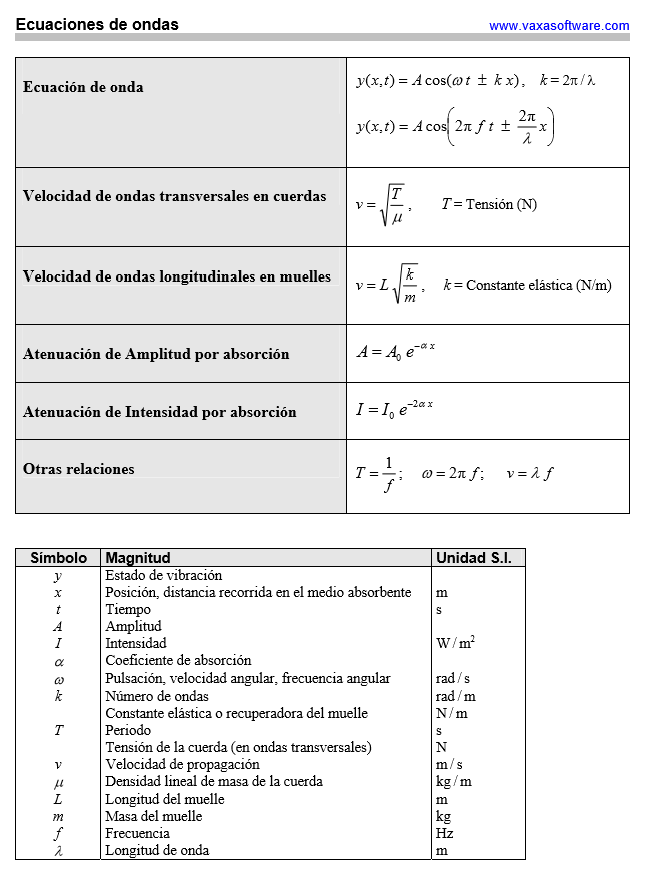
\includegraphics[scale=0.8]{Imagenes/ecOnda}
	\caption{Ecuación de onda}
	\label{fig:ecOnda}
\end{figure}


\begin{equation}
sin x=\frac{e^{ix}-e^{-ix}}{2i}
\end{equation}

Sean:\\

\begin{equation}
\hat{E}(z,t)=E_0\hat{i}e^{i(kz-\omega t)}
\end{equation}

\begin{equation}
\hat{B}(z,t)=B_0\hat{j}e^{i(kz-\omega t)}
\end{equation}

Nota:\\

\begin{equation}
k=\frac{2 \Pi}{\lambda}
\end{equation}

\begin{equation}
\omega = 2 \Pi f
\end{equation}

\begin{equation}
\frac{\omega}{k}=\lambda f = c
\end{equation}

Expresiones de los campos en polarización lineal:\\


\subsection{Propagación de Ondas Electromagnéticas}

\begin{figure}[H]
	\centering
	\begin{tikzpicture}[x={(-10:1cm)},y={(90:1cm)},z={(210:1cm)}]
	% Axes
	\draw (-1,0,0) node[above] {$z$} -- (5,0,0);
	\draw (0,0,0) -- (0,2,0) node[above] {$y$};
	\draw (0,0,0) -- (0,0,2) node[left] {$x$};
	% Propagation
	%\draw[->,ultra thick] (5,0,0) -- node[above] {$c$} (6,0,0);
	% Waves
	\draw[thick] plot[domain=0:4.5,samples=200] (\x,{cos(deg(pi*\x))},0);
	\draw[red,thick] plot[domain=0:4.5,samples=200] (\x,0,{cos(deg(pi*\x))});
	% Arrows
	%\foreach \x in {0.1,0.3,...,4.4} {
	%	\draw[->,help lines] (\x,0,0) -- (\x,{cos(deg(pi*\x))},0);
	%	\draw[->,help lines] (\x,0,0) -- (\x,0,{cos(deg(pi*\x))});
	%		}
	Labels
	\node[above right] at (0,1,0) {$\bm{E}$};
	\node[below] at (0,0,1) {$\bm{B}$};
	\end{tikzpicture}
	
\end{figure}

\subsection{Ley de Faraday}



%$\nabla \times \hat{E}=$
%\[
%\begin{matrix}
%	i & j & k\\
%	$\frac{\partial}{\partial x}$ & $\frac{\partial}{\partial y}$ & $\frac{\partial}{\partial z}$\\
%	$E_0e^{i(kz- \omega t)}$ & 0 & 0  
%\end{matrix}
%\]


El resultado de la matriz anterior es:\\

\begin{equation}
\nabla \times \hat{E}=E_0ik\hat{j}e+-\frac{\partial}{\partial t}(B_0\hat{j}e^{i(kz - \omega t)})=B_0 \omega i \hat{j} e^{i(kt-\omega t)}
\end{equation}

\subsection{Campos Magnético y Eléctrico}

\begin{equation}
\hat{E}=\frac{\hat{F}}{q}
\end{equation}

\begin{equation}
\hat{F_q}=q\hat{v}=\hat{B}
\end{equation}

\begin{equation}
E_E=\frac{1}{2}=cv^2
\end{equation}

\begin{equation}
c=\frac{f_0 A}{z}
\end{equation}

Si $|\hat{E}|$ es constante entonces:\\

\begin{equation}
|\hat{E}|_t=v
\end{equation}

\begin{equation}
w_b=\frac{1}{2}Li^2
\end{equation}

\begin{equation}
|\hat{B}|=\frac{\mu_0 i N}{t}
\end{equation}


\begin{equation}
L=\frac{\mu_0 N^2 A}{t}
\end{equation}

\subsection{Cálculo de la energía}

\begin{equation}
W_{EB}=W_E+W_B=\frac{1}{2}(\frac{f_0 A}{z})(Ez)^2+\frac{1}{2}(\frac{\mu_0 N^2 A}{z})(\frac{B z}{\mu_0 N})^2
\end{equation}

\begin{equation}
dW_{EB}=dW_e+dW_b
\end{equation}

\begin{equation}
dW_{EB}=\frac{1}{2}=f_0AEdt+\frac{1}{2 \mu_0}AB^2dz
\end{equation}


\subsection{Potencia Electromagnética}

\begin{equation}
P_{EB}=\frac{dW_{EB}}{dt}=\frac{1}{2}f_0AEc+\frac{1}{2 \mu_0}AB^2dz
\end{equation}


\subsection{Relación del campo eléctrico y magnético}

\begin{equation}
\frac{E_0}{B_0}=\frac{\omega}{k}=c
\end{equation}

\begin{equation}
s=\frac{P_{EB}}{A}=\frac{1}{2}f_0E^2c+\frac{1}{2_{m_0}}B^2c
\end{equation}

O también si $\frac{E}{B}=c$

\begin{equation}
s= \frac{1}{2}f_0EBc^2+\frac{1}{2 \mu_0}EB=\frac{1}{2 \mu_0}[1+f_0 \mu_0c^2]
\end{equation}

\subsection{Módulo de vector de Poynting}

\begin{equation}
s=\frac{EB}{\mu_0}
\end{equation}

Al final:\\

\begin{equation}
\hat{s}=\frac{\hat{E} \times \hat{B}}{\mu_0}
\end{equation}

\subsection{Irradiancia promedio}

\begin{equation}
|\hat{s}|_{r.m.s.}=\frac{1}{\mu_0}\frac{E_0}{\sqrt{2}} \times \frac{B_0}{\sqrt{2}}=\frac{E_0 B_0}{2 \mu_0} [\frac{W}{m^2}]
\end{equation}

\subsection{Valor RMS}

\begin{equation}
f(t)=\sqrt{\frac{1}{T} \int_0^T f^2(t)dt}
\end{equation}

$T$ es el periodo total de la función a la cual se le quiere sacar su valor RMS.\\

\subsection{Interfaz plana, incidencia oblicua}

\begin{figure}[h!]
	\centering
	\begin{tikzpicture}[]
	% Axes
	%\draw
	\draw (-2.5,0) -- (2.5,0);
	\draw (0,-2.5) -- (0,2.5);
	%azules
	\draw (0,0) [blue,thick]  -- (1.5,1);
	\draw (0,0) [blue,thick]  -- (-1,1.5);
	\draw (0,0) [blue,thick]  -- (-1,-1.5);
	%rojos
	\draw (0.86,0.5) [red,thick]  -- (0.6,1);
	\draw (-0.5,0.86) [red,thick]  -- (0.2,1.5);
	\draw (-0.5,-0.86) [red,thick]  -- (-1,-0.4);
	
	Labels
	\node[above] at (0,2.5) {$y$};
	\node[above] at (2.5,0) {$x$};
	\node[below right] at (0,-2.5) {$n_2$};
	\node[below left] at (0,-2.5) {$n_1$};
	
	\node[green, above] at (1,0) {$\gamma$};
	\node[green, above] at (-0.5,0) {$\beta$};
	\node[green, below] at (-0.5,0) {$\alpha$};
	
	\node[red, above] at (0.6,1) {$\bar{E_{03}}$};
	\node[red, above] at (0.2,1.5) {$\bar{E_{02}}$};
	\node[red, above] at (-1,-0.4) {$\bar{E_{01}}$};
	
	\node[blue, above] at (1.5,1) {$\bar{k_3}$};
	\node[blue, above] at (-1,1.5) {$\bar{k_2}$};
	\node[blue, above] at (-1,-1.5) {$\bar{k_1}$};
	\end{tikzpicture}
	\caption{Onda 2D}
\end{figure}

\begin{eqnarray}
\bar{k_1}=k_1[cos \alpha \hat{i} + sin \alpha \hat{j}]\\
\bar{k_2}=k_2[-cos \beta \hat{i} + sin \beta \hat{j}]\\
\bar{k_3}=k_3[cos \gamma \hat{i} + sin \gamma \hat{j}]
\end{eqnarray}

\begin{eqnarray}
\bar{E_{01}}=E_{01}[-sin \alpha \hat{i} + cos \alpha \hat{j}]\\
\bar{E_{02}}=E_{02}[sin \beta \hat{i} + cos \beta \hat{j}]\\
\bar{E_{03}}=E_{03}[-sin \gamma \hat{j} + cos \gamma \hat{j}]
\end{eqnarray}

$r=x\hat{j}+y\hat{j}$ Entonces:\\

\begin{eqnarray}
\bar{E_1}=\bar{E_{01}}e^{i(\bar{k_1}\bar{r}-\omega t)}=E_{01}[-sin \alpha \hat{i} + cos \alpha \hat{j}] e^{i[k_1(x cos \alpha + y sin \alpha)-\omega t]}\\
\bar{E_2}=\bar{E_{02}}e^{i(\bar{k_2}\bar{r}-\omega t)}=E_{02}[sin \beta \hat{i} + cos \beta \hat{j}] e^{i[k_2(x cos \beta + y sin \beta)-\omega t]}\\
\bar{E_3}=\bar{E_{03}}e^{i(\bar{k_3}\bar{r}-\omega t)}=E_{03}[-sin \gamma \hat{i} + cos \gamma \hat{j}] e^{i[k_3(x cos \gamma + y sin \gamma)-\omega t]}
\end{eqnarray}

Así: $\bar{E_1}=\bar{E_2}+\bar{E_3}$ Condición de frontera $E_{1y}+E_{2y}=E_{3y}$\\

Componente tangencial de $\bar{E}$ Entonces:\\

\begin{eqnarray}
E_{01}cos \alpha e^{ik_1y sin \alpha-i \omega t}*e^{-i \omega t}\\
E_{02}cos \alpha e^{ik_2y sin \beta-i \omega t}*e^{-i \omega t}\\
E_{03}cos \alpha e^{ik_3y sin \gamma-i \omega t}*e^{-i \omega t}
\end{eqnarray}

Nota importante para la simplificación $e^a+e^b=e^c$ implica que $a=b$ y $b=c$\\

\begin{eqnarray}
E_{01}cos \alpha e^{ik_1y sin \alpha-i \omega t}\\
E_{02}cos \alpha e^{ik_2y sin \beta-i \omega t}\\
E_{03}cos \alpha e^{ik_3y sin \gamma-i \omega t}
\end{eqnarray}

Al final: $k_1ysin \alpha=k_2y sin \beta$ implicando que $k_1$ y $k_2$ están en el mismo medio por lo tanto son iguales obteniendo que: $sin \alpha=sin \beta$ y por tanto $\alpha=\beta$ y éste resultado es la $Ley$ $de$ $la$ $reflexión$. Además $k_1ysin\alpha=k_3sin \gamma$ sustituyendo podemos llegar a $La$ $Ley$ $de$ $snell$: $n_1 sin \alpha=n_2 sin \gamma$\\

\section{Formulario}

%\maketitle
\subsection{Constantes}

Velocidad del sonido: $v_{sonido} = 343 [\frac{m}{s}]$\\
Velocidad de la luz: $c = 299 792 458[\frac{m}{s}]$\\
Constante de Planck: $h = 6.62606957*10^-34 [\frac{J}{s}]$\\

%\begin{wrapfigure}{H}{0.5\textwidth}
	%\centering	
	%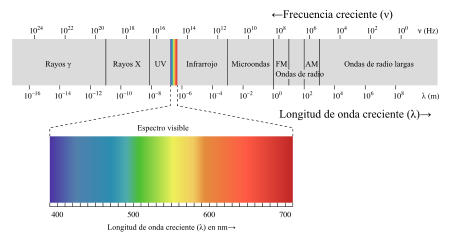
\includegraphics[scale=0.6]{Imagenes/EspectroLuz}
	%\caption{Espectro Electromagnético}
	%\label{fig:EL}
%\end{wrapfigure}

\begin{figure}[H]
		\centering	
	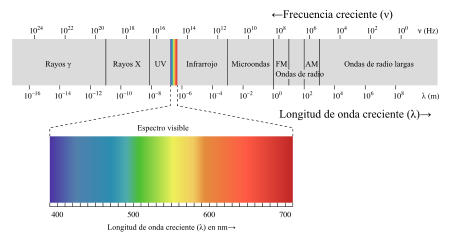
\includegraphics[scale=0.6]{Imagenes/EspectroLuz}
	\caption{Espectro Electromagnético}
	\label{fig:EL}
\end{figure}

\subsection{Ondas}

\begin{equation}
f=\frac{v}{\lambda}
\end{equation}

\begin{equation}
f=\frac{\omega}{2 \Pi}
\end{equation}

\begin{equation}
y(x)=Asin(\omega x+ \phi)
\end{equation}

Donde:\\

\begin{itemize}
	\item $v$ es la velocidad de la onda.
	\item $\lambda$ es la longitud de onda.
	\item $f$ es la frecuencia.
	\item $A$ es la Amplitud de la onda.
	\item $\phi$ es la fase inicial.
	\item $\omega x+ \phi$ es la fase de oscilación.
\end{itemize}

\subsection{Efecto Doppler}


\begin{equation}
v'=v+v_0	
\end{equation}

\begin{equation}
f'=(1+\frac{v_0}{v})
\end{equation}
Donde:\\


\begin{itemize}
	\item $v'$ es la velocidad de las ondas respecto al observador.
	\item $v$ es la velocidad de propagación del sonido.
	\item $v_0$ es la velocidad del observador.
	\item $f'$ es la frecuencia captada por el observador.
\end{itemize}

El observador escuchará un sonido de mayor frecuencia debido que: $(1+\frac{v_0}{v}) \geq 1$.\\

\subsubsection{Observador alejándose de una fuente}

\begin{equation}
f'=f*(1-\frac{v_0}{v})
\end{equation}

\subsubsection{Fuente acercándose a un observador}
En este caso la frecuencia aparente percibida por el observador será mayor que la frecuencia real emitida por la fuente, lo que genera que el observador perciba un sonido más agudo.\\

Por tanto, la longitud de onda percibida para una fuente que se mueve con una velocidad $v_s$, será como se refiere en la ec \ref{fuenteMov}.\\

\begin{equation}
f'=f*(\frac{v}{v-v_s})
\label{fuenteMov}
\end{equation}

\subsubsection{Fuente acercándose a un observador}

\begin{equation}
f'=f*(\frac{1}{1 \pm \frac{v_s}{v}})
\end{equation}

Cuando la fuente se acerque al observador se pondrá un signo (-) en el denominador, y cuando la fuente se aleje se reemplazará por (+).\\
Si el observador y la fuente se mueven al mismo tiempo la ecuación se aprecia en \ref{fuenteObsMov}.\\

\begin{equation}
f^|=f*(\frac{v \pm v_0}{v \pm v_s})
\label{fuenteObsMov}
\end{equation}

\subsection{Ley de Snell}
\begin{equation}
n_1*sin(\theta_1)=n_2*sin(\theta_2)
\end{equation}

\begin{equation}
n=\frac{c}{v}
\end{equation}

Donde:\\

\begin{itemize}
	\item $n_1$ es el índice de refracción del medio 1.
	\item $n_2$ es el índice de refracción del medio 2.
	\item $\theta_1$ es el ángulo con el cual incide la luz.
	\item $\theta_2$ es el ángulo con el cual se desvía la luz en el medio.
\end{itemize}

\begin{figure}[H]
	\centering
	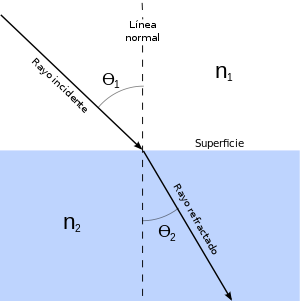
\includegraphics[scale=0.5]{Imagenes/Snell}
	\caption{Ley de Snell}
	\label{fig:Snell}
\end{figure}

\subsection{Ley de Brewster}

\begin{equation}
tan(\theta_b)=\frac{n_2}{n_1}
\end{equation}

Donde:\\

\begin{itemize}
	\item $\theta_b$ es el ángulo de Brewster
	\item $n_1$ es el índice de refracción del medio 1
	\item $n_2$ es el índice de refracción del medio 2
\end{itemize}

\begin{figure}[H]
	\centering
	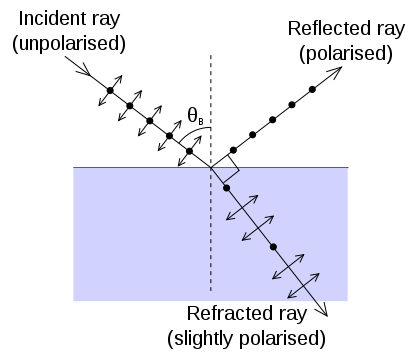
\includegraphics[scale=0.5]{Imagenes/Brewster}
	\caption{Ángulo de Brewster}
	\label{fig:Brewster}
\end{figure}

\subsection{Refracción}

\subsection{Ecuación de refracción de lentes}

\begin{equation}
\frac{n_1}{p}+\frac{n_2}{q}=\frac{n_2-n_1}{R}
\end{equation}

Donde:\\

\begin{itemize}
	\item $p$ es la distancia del objeto al lente
	\item $q$ es la distancia de la imagen al lente
	\item $R$ es el radio de curvatura del lente
\end{itemize}

Una variante de la ley de Snell para un caso particular es:\\
\begin{equation}
tan(\theta_i)=[\frac{sin(\theta_t)-\frac{d}{t}}{cos(\theta_t)}]
\end{equation}

\begin{figure}[H]
	\centering
	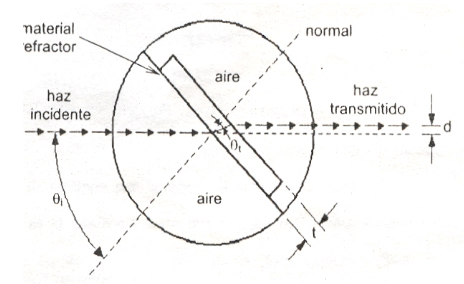
\includegraphics[scale=0.5]{Imagenes/refrac}
	\caption{Refracción}
	\label{fig:refrac}
\end{figure}

\section{Espejos}


\subsubsection{Ecuación de espejos}


\begin{equation}
\frac{1}{p}+\frac{1}{q}=\frac{1}{f}
\end{equation}

\subsubsection{Magnificación}


\begin{equation}
M=-\frac{p}{q}
\end{equation}
Donde:
\begin{itemize}
	\item $p$ es la distancia del objeto al espejo
	\item $q$ es la distancia de la imagen al espejo
	\item $f$ es la distancia del espejo a su foco
\end{itemize}

Para el espejo cóncavo la distancia focal es positiva y para el espejo convexo la distancia focal es negativa.\\

\subsection{Lentes delgadas}
\begin{equation}
\frac{1}{f}=(n-1)*(\frac{1}{R_1}-\frac{1}{R_2})
\end{equation}


Donde:\\

\begin{itemize}
	\item $f$ es la distancia focal
	\item  $n$ es el índice de refrscción del material
	\item  $R_1$ es el Radio de curvatura 1
	\item  $R_2$ es el radio de curvatura 2
\end{itemize}


\subsection{Planck}
\begin{equation}
E=hf
\end{equation}

\begin{equation}
E=\frac{hc}{\lambda}
\end{equation}
Donde:\\

\begin{itemize}
	\item E es la energía de un fotón	
\end{itemize}



%\section{Conclusiones}

%\bibliographystyle{plain}
%\bibliography{Referencias.bib}
%\addbibresource{Referencias.bib}
%\section{Referencias}

%\begin{thebibliography}{widestlabel}
%	\bibitem{MATLABWiki}\textsc{Wikipedia},\textsc{MATLAB},\textsc{https://en.wikipedia.org/wiki/MATLAB},\textit{},WikimediaGroup.
	
 %  \bibitem{Deepl}\textsc{Deepl},\textsc{www.DeepL.com/Translator}
	
	
	
%\end{thebibliography}


\end{document}
